\documentclass{beamer}
\usepackage{listings}
\usepackage{pgf}
\usepackage{verbatim}
\usepackage{hyperref}
%\usepackage[]{algorithm2e}
\usepackage{algorithm,algpseudocode}
%\usepackage{algpseudocode}
%\usepackage{algorithmic}

\pgfdeclareimage[interpolate=true,height=5cm]{data}{data} 
\pgfdeclareimage[interpolate=true,height=5cm]{datamean}{datamean} 
\pgfdeclareimage[interpolate=true,height=4cm]{unit}{unit} 
\pgfdeclareimage[interpolate=true,height=4cm]{Adiag}{Adiag} 
\pgfdeclareimage[interpolate=true,height=5cm]{dataeig}{dataeig} 
\pgfdeclareimage[interpolate=true,height=0.5cm]{digit01}{img/digit_0_1.png} 
\pgfdeclareimage[interpolate=true,height=0.5cm]{digit02}{img/digit_0_2.png} 
\pgfdeclareimage[interpolate=true,height=0.5cm]{digit03}{img/digit_0_3.png} 
\pgfdeclareimage[interpolate=true,height=0.5cm]{digit04}{img/digit_0_4.png} 
\pgfdeclareimage[interpolate=true,height=0.5cm]{digit05}{img/digit_0_5.png} 
\pgfdeclareimage[interpolate=true,height=0.5cm]{digit11}{img/digit_1_1.png} 
\pgfdeclareimage[interpolate=true,height=0.5cm]{digit12}{img/digit_1_2.png} 
\pgfdeclareimage[interpolate=true,height=0.5cm]{digit13}{img/digit_1_3.png} 
\pgfdeclareimage[interpolate=true,height=0.5cm]{digit14}{img/digit_1_4.png} 
\pgfdeclareimage[interpolate=true,height=0.5cm]{digit15}{img/digit_1_5.png} 
\pgfdeclareimage[interpolate=true,height=0.5cm]{digit21}{img/digit_2_1.png} 
\pgfdeclareimage[interpolate=true,height=0.5cm]{digit22}{img/digit_2_2.png} 
\pgfdeclareimage[interpolate=true,height=0.5cm]{digit23}{img/digit_2_3.png} 
\pgfdeclareimage[interpolate=true,height=0.5cm]{digit24}{img/digit_2_4.png} 
\pgfdeclareimage[interpolate=true,height=0.5cm]{digit25}{img/digit_2_5.png} 
\pgfdeclareimage[interpolate=true,height=0.5cm]{digit31}{img/digit_3_1.png} 
\pgfdeclareimage[interpolate=true,height=0.5cm]{digit32}{img/digit_3_2.png} 
\pgfdeclareimage[interpolate=true,height=0.5cm]{digit33}{img/digit_3_3.png} 
\pgfdeclareimage[interpolate=true,height=0.5cm]{digit34}{img/digit_3_4.png} 
\pgfdeclareimage[interpolate=true,height=0.5cm]{digit35}{img/digit_3_5.png} 
\pgfdeclareimage[interpolate=true,height=0.5cm]{digit41}{img/digit_4_1.png} 
\pgfdeclareimage[interpolate=true,height=0.5cm]{digit42}{img/digit_4_2.png} 
\pgfdeclareimage[interpolate=true,height=0.5cm]{digit43}{img/digit_4_3.png} 
\pgfdeclareimage[interpolate=true,height=0.5cm]{digit44}{img/digit_4_4.png} 
\pgfdeclareimage[interpolate=true,height=0.5cm]{digit45}{img/digit_4_5.png} 
\pgfdeclareimage[interpolate=true,height=0.5cm]{digit51}{img/digit_5_1.png} 
\pgfdeclareimage[interpolate=true,height=0.5cm]{digit52}{img/digit_5_2.png} 
\pgfdeclareimage[interpolate=true,height=0.5cm]{digit53}{img/digit_5_3.png} 
\pgfdeclareimage[interpolate=true,height=0.5cm]{digit54}{img/digit_5_4.png} 
\pgfdeclareimage[interpolate=true,height=0.5cm]{digit55}{img/digit_5_5.png} 
\pgfdeclareimage[interpolate=true,height=0.5cm]{digit61}{img/digit_6_1.png} 
\pgfdeclareimage[interpolate=true,height=0.5cm]{digit62}{img/digit_6_2.png} 
\pgfdeclareimage[interpolate=true,height=0.5cm]{digit63}{img/digit_6_3.png} 
\pgfdeclareimage[interpolate=true,height=0.5cm]{digit64}{img/digit_6_4.png} 
\pgfdeclareimage[interpolate=true,height=0.5cm]{digit65}{img/digit_6_5.png} 
\pgfdeclareimage[interpolate=true,height=0.5cm]{digit71}{img/digit_7_1.png} 
\pgfdeclareimage[interpolate=true,height=0.5cm]{digit72}{img/digit_7_2.png} 
\pgfdeclareimage[interpolate=true,height=0.5cm]{digit73}{img/digit_7_3.png} 
\pgfdeclareimage[interpolate=true,height=0.5cm]{digit74}{img/digit_7_4.png} 
\pgfdeclareimage[interpolate=true,height=0.5cm]{digit75}{img/digit_7_5.png} 
\pgfdeclareimage[interpolate=true,height=0.5cm]{digit81}{img/digit_8_1.png} 
\pgfdeclareimage[interpolate=true,height=0.5cm]{digit82}{img/digit_8_2.png} 
\pgfdeclareimage[interpolate=true,height=0.5cm]{digit83}{img/digit_8_3.png} 
\pgfdeclareimage[interpolate=true,height=0.5cm]{digit84}{img/digit_8_4.png} 
\pgfdeclareimage[interpolate=true,height=0.5cm]{digit85}{img/digit_8_5.png} 
\pgfdeclareimage[interpolate=true,height=0.5cm]{digit91}{img/digit_9_1.png} 
\pgfdeclareimage[interpolate=true,height=0.5cm]{digit92}{img/digit_9_2.png} 
\pgfdeclareimage[interpolate=true,height=0.5cm]{digit93}{img/digit_9_3.png} 
\pgfdeclareimage[interpolate=true,height=0.5cm]{digit94}{img/digit_9_4.png} 
\pgfdeclareimage[interpolate=true,height=0.5cm]{digit95}{img/digit_9_5.png} 
\pgfdeclareimage[interpolate=true,height=4.5cm]{twoForMartin}{img/OneforMartinTwoforMartin.jpg} 
\pgfdeclareimage[interpolate=true,height=4.5cm]{knnboundaries}{img/plot_classification_001.png} 
\pgfdeclareimage[interpolate=true,height=2.5cm]{eigdigit1}{img/eigdigit1.png} 
\pgfdeclareimage[interpolate=true,height=2.5cm]{eigdigit2}{img/eigdigit2.png} 
\pgfdeclareimage[interpolate=true,height=2.5cm]{eigdigit3}{img/eigdigit3.png} 
\pgfdeclareimage[interpolate=true,height=2.5cm]{eigdigit4}{img/eigdigit4.png} 
\pgfdeclareimage[interpolate=true,height=2.5cm]{eigdigit5}{img/eigdigit5.png} 
\pgfdeclareimage[interpolate=true,height=2.5cm]{eigdigit6}{img/eigdigit6.png} 
\pgfdeclareimage[interpolate=true,height=8cm]{tcr2}{img/tc_r2.png} 
\pgfdeclareimage[interpolate=true,height=5cm]{kaggle}{img/kaggle.png} 
\pgfdeclareimage[interpolate=true,height=5cm]{kaggle-comp}{img/kaggle-comp.png} 
\pgfdeclareimage[interpolate=true,height=5cm]{kaggle-lead}{img/kaggle-lead.png} 
\pgfdeclareimage[interpolate=true,height=3cm]{alfabeto}{img/AlfabetoMedico1.jpg} 
\pgfdeclareimage[interpolate=true,height=6cm]{parcial1}{img/parcial1.jpg} 
\pgfdeclareimage[interpolate=true,height=3cm]{parcial2}{img/parcial2.jpg} 
\pgfdeclareimage[interpolate=true,height=6cm]{xkcd}{img/xkcd.png} 
\pgfdeclareimage[interpolate=true,height=5cm]{muffin}{img/muffin.jpg}
\pgfdeclareimage[interpolate=true,height=5cm]{angrydog}{img/angrydog.jpg}
\pgfdeclareimage[interpolate=true,height=5cm]{nicedog}{img/nicedog.jpg}
\pgfdeclareimage[interpolate=true,height=8cm]{patente1}{img/Patente1.png}
\pgfdeclareimage[interpolate=true,height=3cm]{patente2}{img/Patente2.jpg}
\pgfdeclareimage[interpolate=true,height=7cm]{confussion}{img/confussion.png}
\pgfdeclareimage[interpolate=true,height=5cm]{eigen}{img/eigen.png}



\begin{document}
\title{Trabajo Pr\'actico 2 \\ \emph{Reconocimiento de d\'igitos}}   
\author{M\'etodos Num\'ericos} 
%\titlegraphic{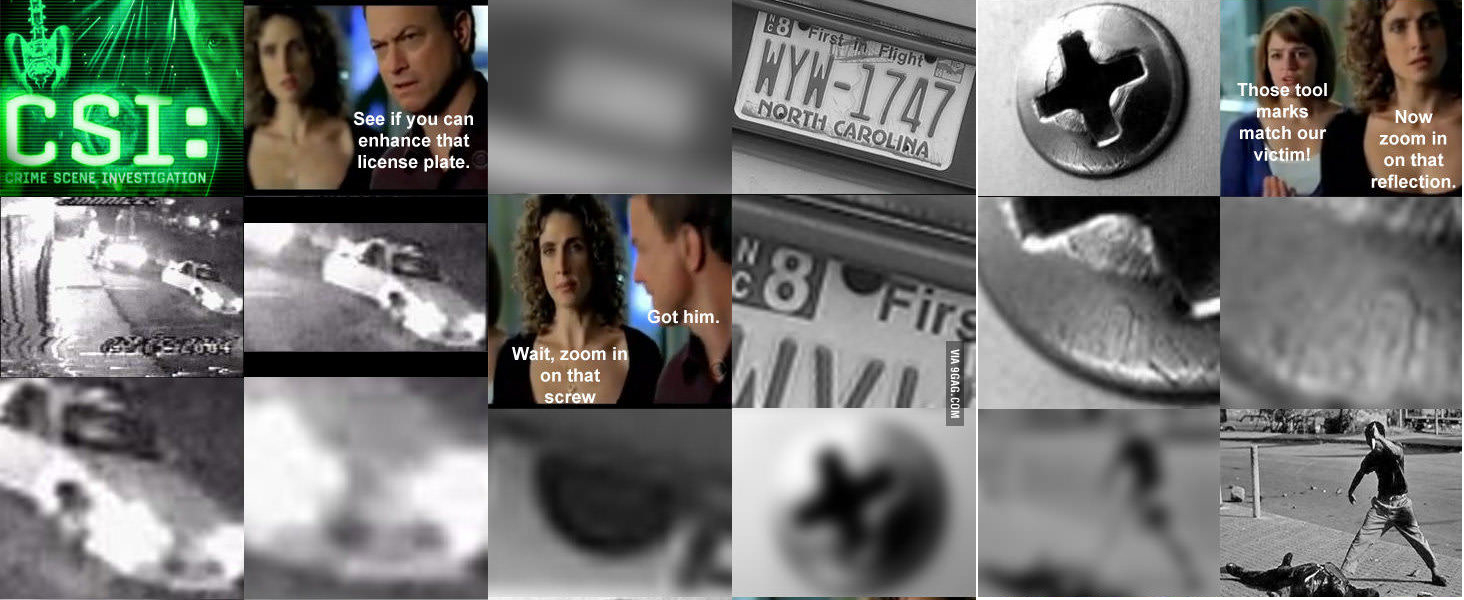
\includegraphics[width=11cm]{img/csihor.jpg}}
\date{Segundo cuatrimestre - 2020} 
%\lstset{language=C}
\lstdefinestyle{customc}{
 belowcaptionskip=1\baselineskip,
 breaklines=true,
 language=C,
 showstringspaces=false,
 basicstyle=\footnotesize,
 keywordstyle=\color{blue!40!black},
 commentstyle=\tiny\color{purple!40!black},
 stringstyle=\color{orange},
}
\lstset{style=customc}

\frame{\titlepage} 
%\frame{\frametitle{Outline}\tableofcontents} 

\frame{
\frametitle{Antes de pasar al TP2...}
\framesubtitle{D\'onde estamos y qu\'e vimos hasta ahora}

\begin{itemize}
\item Errores num\'ericos.
\item Resoluci\'on de sistema lineales. (EG, LU, SDP)
\item Aplicaci\'on de resoluci\'on de sistemas (Rankings deportivos y otros rankings).
\item Aplicaciones de Cholesky a generaci\'on de variables.
\item C\'omo experimentar, tanto a nivel metodol\'ogico como a nivel implementaci\'on.
\end{itemize}

}

\frame{
\frametitle{Subiendonos a la ola: un TP de Machine Learning}

\pause
\begin{minipage}{0.45\textwidth}
\begin{center}
\pgfuseimage{xkcd}
\end{center}
\end{minipage}
~
\pause
\begin{minipage}{0.45\textwidth}
\begin{center}
\pgfuseimage{muffin}
\end{center}
\end{minipage}
}

\frame{
\frametitle{En realidad ya estabamos en la ola}
\framesubtitle{Reacciones populares}
\begin{minipage}{0.45\textwidth}
\begin{center}
\vspace{15pt}
M\'etodos num\'ericos

\pgfuseimage{angrydog}

Norma matricial, n\'umero de condici\'on, factorizaci\'on de matrices, distancia de un punto a un subespacio
\end{center}
\end{minipage}
~
\begin{minipage}{0.45\textwidth}
\begin{center}
Machine learning

\pgfuseimage{nicedog}

Data scientist, Big data, Deep learning, Data guru ninja visionary
\end{center}
\end{minipage}
}


\frame{
\frametitle{Trabajo Pr\'actico 2}
\framesubtitle{Reconocimiento de d\'igitos - Aplicaciones}
\begin{minipage}{0.45\textwidth}
\begin{center}
\pgfuseimage{patente1}
\end{center}
\end{minipage}
~
\begin{minipage}{0.45\textwidth}
\begin{center}
\pgfuseimage{patente2}
\end{center}
\end{minipage}
}

\frame{
\frametitle{Trabajo Pr\'actico 2}
\framesubtitle{Reconocimiento de d\'igitos}

\begin{itemize}
\item Datos: base de datos etiquetada de im\'agenes de d\'igitos manuscritos (0-9) tomadas de una forma particular.
\item Objetivo: dada una nueva imagen de un d\'igito, ?`A cu\'al corresponde?
\end{itemize}

\begin{minipage}{0.6\linewidth}
\begin{center}
\begin{minipage}{0.05\linewidth}
0:
\end{minipage}
\begin{minipage}{0.5\linewidth}
\pgfuseimage{digit01}
~
\pgfuseimage{digit02}
~
\pgfuseimage{digit03}
~
\pgfuseimage{digit04}
~
\pgfuseimage{digit05}
\end{minipage}

\begin{minipage}{0.05\linewidth}
1:
\end{minipage}
\begin{minipage}{0.5\linewidth}
\pgfuseimage{digit11}
~
\pgfuseimage{digit12}
~
\pgfuseimage{digit13}
~
\pgfuseimage{digit14}
~
\pgfuseimage{digit15}
\end{minipage}

\begin{minipage}{0.05\linewidth}
2:
\end{minipage}
\begin{minipage}{0.5\linewidth}
\pgfuseimage{digit21}
~
\pgfuseimage{digit22}
~
\pgfuseimage{digit23}
~
\pgfuseimage{digit24}
~
\pgfuseimage{digit25}
\end{minipage}

\begin{minipage}{0.05\linewidth}
3:
\end{minipage}
\begin{minipage}{0.5\linewidth}
\pgfuseimage{digit31}
~
\pgfuseimage{digit32}
~
\pgfuseimage{digit33}
~
\pgfuseimage{digit34}
~
\pgfuseimage{digit35}
\end{minipage}

\begin{minipage}{0.05\linewidth}
4:
\end{minipage}
\begin{minipage}{0.5\linewidth}
\pgfuseimage{digit41}
~
\pgfuseimage{digit42}
~
\pgfuseimage{digit43}
~
\pgfuseimage{digit44}
~
\pgfuseimage{digit45}
\end{minipage}

\begin{minipage}{0.05\linewidth}
5:
\end{minipage}
\begin{minipage}{0.5\linewidth}
\pgfuseimage{digit51}
~
\pgfuseimage{digit52}
~
\pgfuseimage{digit53}
~
\pgfuseimage{digit54}
~
\pgfuseimage{digit55}
\end{minipage}

\begin{minipage}{0.05\linewidth}
6:
\end{minipage}
\begin{minipage}{0.5\linewidth}
\pgfuseimage{digit61}
~
\pgfuseimage{digit62}
~
\pgfuseimage{digit63}
~
\pgfuseimage{digit64}
~
\pgfuseimage{digit65}
\end{minipage}

\begin{minipage}{0.05\linewidth}
7:
\end{minipage}
\begin{minipage}{0.5\linewidth}
\pgfuseimage{digit71}
~
\pgfuseimage{digit72}
~
\pgfuseimage{digit73}
~
\pgfuseimage{digit74}
~
\pgfuseimage{digit75}
\end{minipage}

\begin{minipage}{0.05\linewidth}
8:
\end{minipage}
\begin{minipage}{0.5\linewidth}
\pgfuseimage{digit81}
~
\pgfuseimage{digit82}
~
\pgfuseimage{digit83}
~
\pgfuseimage{digit84}
~
\pgfuseimage{digit85}
\end{minipage}

\begin{minipage}{0.05\linewidth}
9:
\end{minipage}
\begin{minipage}{0.5\linewidth}
\pgfuseimage{digit91}
~
\pgfuseimage{digit92}
~
\pgfuseimage{digit93}
~
\pgfuseimage{digit94}
~
\pgfuseimage{digit95}
\end{minipage}
\end{center}
\end{minipage}
\begin{minipage}{0.35\linewidth}
\begin{block}{Problema a resolver}
Recibimos un nuevo d\'igito manuscrito, ?`Podemos determinar autom\'aticamente a cu\'al pertenece?
\end{block}
\end{minipage}

}

\frame{
\frametitle{Reconocimiento de d\'igitos}
\framesubtitle{Contexto}
{\small
\begin{block}{Objetivo}
Desarrollar (no solo en t\'erminos de implementaci\'on) un \emph{clasificador} que permita reconocer d\'igitos manuscritos.
\end{block}

\begin{block}{Contexto}
\begin{itemize}
\item Disponemos de una base de datos etiquetada (train), y un conjunto de datos para los que no conocemos cu\'al es su etiqueta (test). Este \'ultimo nos permitir\'a evaluar como se comporta nuestro clasificador.
\item Consideramos la base MNIST, en la versi\'on utilizada en \emph{Kaggle}. 42k d\'igitos en train, 18k d\'igitos en test.
\item Cada d\'igito es una imagen en escala de grises de $28\times 28$.
\end{itemize}
\end{block}
}
}


\frame{
\frametitle{Reconocimiento de d\'igitos}
\framesubtitle{Vecino m\'as cercano}

\begin{block}{Idea general (caso particular reconocimiento d\'igitos)}
\begin{itemize}
\item Consideramos cada imagen como un vector $x_i \in \mathbb{R}^{m}$, $m = 28\times 28$, $i = 1,\dots,n$. Para las im\'agenes en la base de datos, sabemos adem\'as a que clase pertenece.
\item Cuando llega una nueva imagen de un d\'igito $z$, con el mismo formato, recorremos toda la base y buscamos aquella que minimice
\begin{displaymath}
{\arg\min}_{i = 1,\dots,n} \|z - x_i \|_2
\end{displaymath}
Luego, le asignamos la clase del representante seleccionado.
\end{itemize}
\end{block}

\begin{block}{Generalizaci\'on}
Considerar m\'as de un vecino.
\end{block}

}


\frame{
\frametitle{Reconocimiento de d\'igitos}
\framesubtitle{Vecinos m\'as cercanos: $kNN$}

\begin{itemize}
\item Consideramos los $k$ vecinos m\'as cercanos.
\item Entre ellos hacemos una votaci\'on, eligiendo como clase la \emph{moda} del conjunto. En otras palabras, hacemos una votaci\'on y se elige aquella clase con m\'as votos.

\begin{center}
\pgfuseimage{twoForMartin}
\end{center}
\end{itemize}

}

\frame{
\frametitle{Reconocimiento de d\'igitos}
\framesubtitle{$kNN$: Ejemplo de clasificaci\'on y definici\'on de fronteras}

\begin{minipage}{0.5\linewidth}
\pgfuseimage{knnboundaries}
\end{minipage}
\begin{minipage}{0.45\linewidth}
{\small
\begin{block}{Algunos pros \& cons}
\begin{itemize}
\item[+] Es conceptualmente simple. 
\item[+] Funciona bien en general para dimensiones bajas, y puede ser utilizado con pocos ejemplos.
\item[-] Sufre de \emph{La maldici\'on de la dimensionalidad.}
\item[-] La clasificaci\'on puede ser lenta dependiendo del contexto.
\end{itemize}
\end{block}
}
\end{minipage}


{\scriptsize Imagen tomada de \textsc{scikit-learn.org}}
}


\frame{
\frametitle{An\'alisis de Componentes Principales}
\framesubtitle{Ejemplo datos en $\mathbb{R}^2$}

Sean $x^{(1)},x^{(2)},\dots,x^{(n)}$ una secuencia de $n$ datos, con $x^{(i)} \in \mathbb{R}^2$.

{\tiny
\begin{minipage}{0.4\linewidth}
\begin{displaymath}
X = 
\begin{bmatrix}
x^{(1)^t} \\
x^{(2)^t} \\
x^{(3)^t} \\
x^{(4)^t} \\
x^{(5)^t} \\
x^{(6)^t} \\
\vdots \\
x^{(n)^t} \\
\end{bmatrix}
=
\begin{bmatrix}
26.4320 &  27.7740 \\
26.8846 &  26.5631 \\
23.3309 &  26.6983 \\
30.6387 &  31.5619 \\
30.5171 &  30.8993 \\
45.6364 &  36.6035 \\
\vdots  &  \vdots \\		
16.0650 &  24.0210 \\
\end{bmatrix}
\end{displaymath}
\end{minipage}
~
\begin{minipage}{0.55\linewidth}
\pgfuseimage{data}
\end{minipage}
}
}

\frame{
\frametitle{An\'alisis de Componentes Principales}
\framesubtitle{Ejemplo datos en $\mathbb{R}^2$}
\begin{minipage}{0.4\linewidth}
{\footnotesize
\begin{displaymath}
X = 
\begin{bmatrix}
26.4320 &  27.7740 \\
26.8846 &  26.5631 \\
23.3309 &  26.6983 \\
30.6387 &  31.5619 \\
30.5171 &  30.8993 \\
45.6364 &  36.6035 \\
\vdots  &  \vdots \\		
16.0650 &  24.0210 \\
\end{bmatrix}
\end{displaymath}
}
\end{minipage}
~
\begin{minipage}{0.55\linewidth}
\pgfuseimage{datamean}
\end{minipage}

\begin{minipage}{0.45\linewidth}
{\small
\underline{Media:}

$\mu = \frac{1}{n}(x^{(1)} + \dots + x^{(n)})$

$\mu = (29.3623,29.7148)$
}
\end{minipage}
~
\begin{minipage}{0.45\linewidth}
{\small
\underline{Varianza de una variable $x_k$:} Medida para la dispersi\'on de los datos.

$\sigma^2 = \frac{1}{n-1}\sum_{i = 1}^n (x_k^{(i)} - \mu_k)^2$

$\sigma_{x_1}^2 = 66.2134,~\sigma_{x_2}^2 = 12.5491$
}
\end{minipage}
}

\frame{
\frametitle{An\'alisis de Componentes Principales}
\framesubtitle{Ejemplo datos en $\mathbb{R}^2$ - Covarianza}

\begin{minipage}{0.4\linewidth}
{\footnotesize
\begin{displaymath}
X = 
\begin{bmatrix}
26.4320 &  27.7740 \\
26.8846 &  26.5631 \\
23.3309 &  26.6983 \\
30.6387 &  31.5619 \\
30.5171 &  30.8993 \\
45.6364 &  36.6035 \\
\vdots  &  \vdots \\		
16.0650 &  24.0210 \\
\end{bmatrix}
\end{displaymath}
}
\end{minipage}
~
\begin{minipage}{0.55\linewidth}
{\small
\underline{Covarianza:} Medida de cu\'anto dos variables var\'ian de forma similar. Variables con mayor covarianza
inducen la presencia de cierta dependencia o relaci\'on.
}
\end{minipage}

\begin{displaymath}
\sigma_{x_j x_k} = \frac{1}{n-1}\sum_{i = 1}^n (x_j^{(i)} - \mu_j)(x_k^{(i)} - \mu_k)
\end{displaymath}
}

\frame{
\frametitle{An\'alisis de Componentes Principales}
\framesubtitle{Ejemplo datos en $\mathbb{R}^2$ - Covarianza}

Dadas $n$ observaciones de dos variables $x_k$, $x_j$, y $v = (1,\dots,1)^t$:

\begin{displaymath}
\sigma_{x_j x_k} = \frac{1}{n-1}\sum_{i = 1}^n (x_j^{(i)} - \mu_j)(x_k^{(i)} - \mu_k) = \frac{1}{n-1}(x_k - \mu_k
v)^t(x_j - \mu_jv) 
\end{displaymath}

Matriz de Covarianza:

\begin{minipage}{0.4\linewidth}
{\footnotesize
\begin{displaymath}
X = 
\begin{bmatrix}
26.4320 - \mu_1 &  27.7740 - \mu_2 \\
26.8846 - \mu_1 &  26.5631 - \mu_2 \\
23.3309 - \mu_1 &  26.6983 - \mu_2 \\
30.6387 - \mu_1 &  31.5619 - \mu_2 \\
30.5171 - \mu_1 &  30.8993 - \mu_2 \\
45.6364 - \mu_1 &  36.6035 - \mu_2 \\
\vdots  &  \vdots \\		
16.0650 - \mu_1 &  24.0210 - \mu_2 \\
\end{bmatrix}
\end{displaymath}
}
\end{minipage}
~
\begin{minipage}{0.55\linewidth}
{\footnotesize
\begin{displaymath}
M_X = \frac{1}{n-1} X^t X = \begin{bmatrix}
\sigma_{x_1 x_1} & \sigma_{x_1 x_2} \\
\sigma_{x_1 x_2} & \sigma_{x_2 x_2} \\
\end{bmatrix}
\end{displaymath}
\begin{displaymath}
~~~~~~~~~~~~~~~~~~~~~~= \begin{bmatrix}
\sigma_{x_1}^2 & \sigma_{x_1 x_2} \\
\sigma_{x_1 x_2} & \sigma_{x_2}^2 \\
\end{bmatrix}
\end{displaymath}

\begin{displaymath}
M_X = \begin{bmatrix}
 66.2134 &  27.1263 \\
 27.1263 &  12.5491 \\
\end{bmatrix}
\end{displaymath}
}
\end{minipage}
}

\frame{
\frametitle{?`C\'omo expresar mejor nuestros datos?}

\begin{block}{Objetivo}
Buscamos una transformaci\'on de los datos que disminuya la redundancia (es decir, disminuir la covarianza).
\end{block}

\begin{itemize}
\item Cambio de base: $\hat{X}^t = P X^t$.
\item C\'omo podemos hacerlo? Diagonalizar la matriz de covarianza. Esta matriz tiene la varianza de cada variable en la
diagonal, y la covarianza en las restantes posiciones. Luego, al diagonalizar buscamos variables que tengan covarianza
cero entre s\'i y la mayor varianza posible.
\end{itemize}


}

\frame{
\frametitle{Autovalores y Autovectores}

\begin{block}{Definici\'on}
Sea $A \in \mathbb{R}^{n \times n}$. Un \emph{autovector} de $A$ es un vector no nulo tal que $Ax = \lambda x$, para algun
escalar $\lambda$. Un escalar $\lambda$ es denominado \emph{autovalor} de $A$ si existe una soluci\'on no trivial $x$
del sistema $Ax = \lambda x$. En este caso, $x$ es llamado \emph{autovector asociado a $\lambda$}.
\end{block}

Consideramos:

\begin{displaymath}
A = \begin{bmatrix}
3 & -2 \\
1 & 0 \\
\end{bmatrix},
u = \begin{bmatrix}
-1 \\
1 \\
\end{bmatrix},
v = \begin{bmatrix}
2 \\
1 \\
\end{bmatrix}
\end{displaymath}

\begin{displaymath}
Au = \begin{bmatrix}
-5 \\
-1 \\
\end{bmatrix},
Av = \begin{bmatrix}
4\\
2\\
\end{bmatrix}
= 2 \begin{bmatrix}
2\\
1\\
\end{bmatrix}
= 2v
\end{displaymath}

Gr\'aficamente....$A$ s\'olo estira (o encoge) el vector $v$.
}

\frame{
\frametitle{Diagonalizaci\'on}

En muchos casos, la presencia de autovectores-autovalores puede ser utilizada para encontrar una factorizaci\'on $A =
PDP^{-1}$, donde $D$ es una matriz diagonal.

\begin{block}{Intuici\'on}
Podemos encontrar una base donde la transformaci\'on lineal $A$ se comporta como si fuese diagonal.
\end{block}

\begin{block}{Observaci\'on}
No toda matriz $A \in \mathbb{R}^{n \times n}$ es diagonalizable.
\end{block}

\begin{block}{Teorema}
Una matriz $A\in \mathbb{R}^{n \times n}$ es diagonalizable s\'i y solo s\'i $A$ tiene $n$ autovectores linealmente
independientes (las columnas de $P$).
\end{block}

\begin{block}{Teorema}
Si $A \in \mathbb{R}^{n \times n}$ es sim\'etrica, entonces existe una base ortonormal de autovectores
$\{v_1,\dots,v_n\}$ asociados a $\lambda_1,\dots,\lambda_n$. 
\end{block}

Consecuencia: Existe $P$, y $P^{-1} = P^t$. Luego, $A = PDP^t$.
}

\frame{
\frametitle{C\'alculo de autovalores/autovectores}

\begin{itemize}
\item Vamos a necesitar calcular los autovectores $v$ de una matriz para poder calcular las transformaci\'ones de los m\'etodos que estamos viendo.

\item Consideremos $A^tA$, y supongamos $\lambda_1 > \lambda_2 > \dots > \lambda_k$. $A^tA$ es sim\'etrica y
semidefinida positiva. 
\item Podemos considerar el \underline{M\'etodo de la Potencia} para calcular $\lambda_1$ y $v_1$.
\begin{enumerate}
\item MetodoPotencia($B$,$x_0$,niter)
\item ~~~~$v \gets x_0$.
\item ~~~~Para $i = 1,\dots,niter$
\item ~~~~~~~~$v \gets \frac{Bv}{||Bv||}$
\item ~~~~Fin Para
\item ~~~~$\lambda \gets \frac{v^tBv}{v^tv}$
\item ~~~~Devolver $\lambda, v$.
\end{enumerate}
\end{itemize}
}

\frame{
\frametitle{C\'alculo de autovalores/autovectores}
Una vez que tenemos $\lambda_1$ y $v_1$, como seguimos?

\begin{block}{Deflaci\'on}
Sea $B \in \mathbb{R}^{n \times n}$ una matriz con autovalores distintos $|\lambda_1| > |\lambda_2| > \dots >
|\lambda_n|$ y
una base ortonormal de autovectores. Entonces, la matriz $B - \lambda_1 v_1 v_1^t$ tiene autovalores
$0,\lambda_2,\dots,\lambda_n$ con autovectores asociados $v_1,\dots,v_n$.
\end{block}
\begin{itemize}
\item $(B - \lambda_1 v_1 v_1^t)v_1 = B v_1 - \lambda_1 v_1 (v_1^t v_1) = \lambda_1 v_1 - \lambda_1 v_1 = 0 v_1$.
\item $(B - \lambda_1 v_1 v_1^t)v_i = B v_i - \lambda_1 v_1 (v_1^t v_i) = \lambda_i v_i$.
\end{itemize}

\begin{block}{Observaci\'on}
En nuestro caso, no hace falta que todos los autovalores tengan magnitudes distintas.
\end{block}
}

\frame{
\frametitle{?`C\'omo expresar mejor nuestros datos?}
{\small
\begin{itemize}
\item Cambio de base: $\hat{X}^t = PX^t$.

Sea $P$ ortogonal y $M_{\hat{X}}$ la matriz de covarianza de $\hat{X}$.
\begin{eqnarray*}
M_{\hat{X}} & = & \frac{1}{n-1}\hat{X}^t\hat{X}\\
& = & \frac{1}{n-1}(PX^t)(XP^t) \\
& = & P \frac{X^tX}{n-1} P^t \\
& = & P M_X P^t
\end{eqnarray*}
\item $M_X$ es sim\'etrica, entonces existe $V$ ortogonal tal que $M_X = VDV^t$.
\begin{eqnarray*}
M_{\hat{X}} & = & PM_XP^t\\
& = & P(VDV^t)P^t ~~~~~~~ \textrm{tomamos } P = V^ t\\
& = & (V^tV)D(VV^t) = D
\end{eqnarray*}
\end{itemize}
}
}


\frame{
\frametitle{?`C\'omo expresar mejor nuestros datos?}
\framesubtitle{Volvemos al ejemplo}
{\small
\begin{eqnarray*}
M_X & = & \begin{bmatrix}
 66.2134 &  27.1263 \\
 27.1263 &  12.5491 \\
\end{bmatrix}\\
& = & 
\underbrace{\begin{bmatrix}
0.9228 & -0.3852\\
0.3852 &  0.9228\\
\end{bmatrix}}_{V}
\underbrace{\begin{bmatrix}
77.5362 & 0\\
0 & 1.2263\\
\end{bmatrix}}_{D = M_{\hat{X}}}
\underbrace{\begin{bmatrix}
0.9228 & 0.3852\\
-0.3852 &  0.9228\\
\end{bmatrix}}_{V^t}
\end{eqnarray*}
}

\begin{center}
\pgfuseimage{dataeig}
\end{center}
}

\frame{
\frametitle{An\'alisis de Componentes Principales}
\framesubtitle{Resumen hasta ac\'a}
{\small
\begin{itemize}
\item Tenemos $n$ muestras de $m$ variables.
\item Calculamos el vector $\mu$ que contiene la media de cada de una las variables. 
\item Construimos la matriz $X \in \mathbb{R}^{n \times m}$ donde cada muestra corresponde a una fila de $X$ y tienen
media cero (i.e., $x^{(i)} := (x^{(i)} - \mu)/\sqrt{n-1}$).
\item Diagonalizamos la matriz de covarianzas $M_X$. La matriz $V$ (ortogonal) contiene los autovectores de $M_X$.
\end{itemize}

Propiedades del cambio de base
\begin{itemize}
\item Disminuye redundancias.
\item El cambio de base $\hat{X}^t = PX^t = V^tX^t$ asigna a cada muestra un nuevo \emph{nombre} mediante un cambio de
coordenadas.
\item Las columnas de $V$ (autovectores de $M_X$) son las componentes principales de los datos.
\item En caso de $m$ grande, es posible tomar s\'olo un subconjunto de las componentes principales para estudiar (i.e.,
aquellas que capturen mayor proporci\'on de la varianza de los datos). 
\end{itemize}
}
}


\begin{comment}
\frame{
\frametitle{An\'alisis de Componentes Pricipales}
\framesubtitle{Utilizando la descomposici\'on en valores singulares}
{\small
%En la pr\'actica, PCA utiliza la descomposici\'on SVD.

\begin{block}{Teorema (Descomposici\'on SVD)}
Sea $A \in \mathbb{R}^{n \times m}$ una matriz con rango $r$. Entonces, existe $\Sigma \in \mathbb{R}^{n \times m}$, $U
\in \mathbb{R}^{n \times n}$ y $V \in \mathbb{R}^{m \times m}$ ortogonales tales que $A = U\Sigma V^t$, y adem\'as 
\begin{displaymath}
\Sigma = \begin{bmatrix}
D & 0 \\
0 & 0 \\
\end{bmatrix}
\end{displaymath}
\noindent con $D \in \mathbb{R}^{r \times r}$ una matriz diagonal con $d_{ii} = \sigma_i > 0$ los valores singulares,
$\sigma_i \ge \sigma_{i+1}$.
\end{block}

\begin{block}{Observaci\'on}
Toda matriz tiene descomposici\'on SVD.
\end{block}

\begin{block}{Qui\'en es qui\'en}
\begin{itemize}
\item $\sigma_i = \sqrt{\lambda_i}$, $\lambda_i$ autovalor de $A^tA$.
\item $V = [v_1 v_2 \dots v_m]$, $A^tA v_i = \lambda_i v_i$.
\item $u_i = \frac{1}{\sigma_i}Av_i$, $i = 1,\dots,r$ (el resto, extender a base ortonormal).
\end{itemize}
\end{block}
}
}

\frame{
\frametitle{An\'alisis de Componentes Pricipales}
\framesubtitle{Utilizando la descomposici\'on en valores singulares}
\begin{itemize}
\item Tenemos $n$ muestras de $m$ variables.
\item Calculamos el vector $\mu$ que contiene la media de cada de una las variables. 
\item Construimos la matriz $X \in \mathbb{R}^{n \times m}$ donde cada muestra corresponde a una fila de $X$ y tienen
media cero (i.e., $x^{(i)} := x^{(i)} - \mu$).
\item Definimos $A = X/\sqrt{n-1}$.
\item Sea $A = U\Sigma V^t$.
\item $M_X = A^tA = V \Sigma^t U^t U \Sigma V^t = V \Sigma^t \Sigma V^t$. 
\item Las columnas de $V$ contienen los autovectores de $M_X$.
\end{itemize}
}

\frame{
\frametitle{Reconocimiento de d\'igitos}
\framesubtitle{Aplicando PCA}
{\small
\begin{itemize}
\item Tenemos una base de datos de $n$ im\'agenes con caras de personas. Cada imagen es una muestra. 
\item Cada imagen tiene $h \times w = m$ p\'ixeles, donde cada p\'ixel corresponde a una variable. Disponemos cada imagen
como un vector $x^{(i)} \in \mathbb{R}^{m}$.\\ Obs: Una base, dos resoluciones: $112\times 92$, $28 \times 23$.
\item Calculamos el vector $\mu = (x^{(1)} + \dots + x^{(n)})/n$ que contiene la media de cada de una las variables. 
\item Definimos $X \in \mathbb{R}^{n \times m}$, y $A = X/\sqrt{n-1}$.
\item El vector $\frac{(x^{(i)} - \mu)^t}{\sqrt{n-1}}$ es la i-\'esima fila de $A$.
\item Calculamos $A = U\Sigma V^t$ la descomposici\'on SVD de $A$ (en la pr\'actica, solo nos interesa $V$
ya que tiene los autovectores de $M_X$).
\end{itemize}
\small}
}
\end{comment}

\frame{
\frametitle{Reconocimiento de d\'igitos}
\framesubtitle{Autod\'igitos (Eigendigits)}

Los primeros 6 autovectores en $V$.

\begin{center}
\pgfuseimage{eigdigit1}
\pgfuseimage{eigdigit2}
\pgfuseimage{eigdigit3}

\pgfuseimage{eigdigit4}
\pgfuseimage{eigdigit5}
\pgfuseimage{eigdigit6}
\end{center}
}


\frame{
\frametitle{Reconocimiento de d\'igitos}
\framesubtitle{?`C\'omo reconocemos un d\'igito?}
{\small
\begin{block}{Idea}
\begin{itemize}
\item Utilizar el cambio de base, transformando cada imagen convenientemente. 
\item Reducir la dimensi\'on de los datos utilizando s\'olo algunas de las nuevas variables (eligiendo aquellas que
capturan una fracci\'on mayor de la varianza).
\end{itemize}
\end{block}
\begin{block}{Procedimiento}
\begin{itemize}
\item \underline{Reducci\'on de la dimensi\'on:} par\'ametro de entrada que indica cu\'antas componentes principales considerar,
$\alpha$. Es decir, tomaremos $\bar{V} = [v_1~v_2~\dots~v_{\alpha}]$.
\item \underline{Tranformaci\'on caracter\'istica:} Aplicamos el cambio de base a cada muestra $x^{(i)}$, definimos
$tc(x^{(i)}) = \bar{V}^t x^{(i)} = (v_1^t x^{(i)},\dots,v_{\alpha}^t x^{(i)})$.
\end{itemize}
\end{block}
}
}


\frame{
\frametitle{Reconocimiento de d\'igitos}
\framesubtitle{Transformaci\'on + Reducci\'on ($k = 2$)}
\begin{center}
\pgfuseimage{tcr2}
\end{center}
}


\frame{
\frametitle{Reconocimiento de d\'igitos}
\framesubtitle{?`C\'omo reconocemos un d\'igito?}
Finalmente, dada una imagen de un d\'igito que no se encuentra en la base:

\begin{itemize}
\item Vectorizamos la imagen en $x^* \in \mathbb{R}^m$.
\item Definimos $\bar{x}^* = (x^* - \mu)/\sqrt{n-1}$. 
\item Aplicamos la transformaci\'on caracter\'istica, $tc(\bar{x}^*)$ y buscamos (de alguna manera) a que d\'igito 
pertenece.
\end{itemize}


\begin{block}{Pregunta:}
Sugerencias para buscar a qu\'e d\'igito pertenece?
\end{block}

}


\frame{
\frametitle{Reconocimiento de d\'igitos}
\framesubtitle{Metodolog\'ia de evaluaci\'on}

Elegimos un numero de vecinos $k$ (adicionalmente un n\'umero $\alpha$ o $\gamma$ de componentes). Como evaluamos si el m\'etodo funciona?

\begin{itemize}
\item Como medimos la efectividad del m\'etodo?
\pause
\item Tiene sentido probarlo sobre la base de training?
\pause
\item De alguna forma defino una instancia, pruebo todas las combinaciones de par\'ametros sobre la misma. Es correcto? Puede surgir alg\'un problema?
\end{itemize}
\pause
\begin{block}{Idea}
Utilizar la base de entrenamiento convenientemente para estimar y proveer suficiente evidencia respecto a la efectividad del m\'etodo. 
\end{block}

}

\frame{
\frametitle{Midiendo la efectividad - Matriz de confusi\'on}

\begin{center}
\pgfuseimage{confussion}
\end{center}
}

\frame{
\frametitle{M\'etricas}

\begin{itemize}

\item \textbf{Accuracy}: Los aciertos totales sobre los casos totales. En t\'erminos de la matriz de confusi\'on, sumar la diagonal dividido la suma de todas las celdas.

\item \textbf{Precision}: Aciertos relativos dentro de una clase. Dada una clase $i$, $\frac{tp_i}{tp_i+fp_i}$.

 La $precision$ en el caso de un clasificador de muchas clases, se define como el promedio de las $precision$ para cada una de las clases.

\item \textbf{Recall}: M\'etrica para medir los reconocimientos dentro de una clase. Dada una clase $i$, $\frac{tp_i}{tp_i+fn_i}$.

\end{itemize}
}

\frame{
\frametitle{M\'etricas}
\begin{itemize}
\item \textbf{F1-Score}: Dado que $precision$ y $recall$ son dos medidas importantes que no necesariamente tienen la misma calidad para un mismo clasificador, se define la m\'etrica F1 para medir un compromiso entre el $recall$ y la $precision$. La m\'etrica $F1$ se define como $2*precision*recall / (precision + recall) $.


\item \textbf{Kappa de Cohen}: Es una medida para indicar cu\'anto concuerdan dos clasificadores sobre un mismo set de datos. Dicha medida se define como $\kappa = (p_o - p_a)/(1 - p_a)$. Donde $p_o$ es la probabilidad observada de que los dos clasificadores concuerden y $p_a$ es la probabilidad aleatoria de que lo hagan.

Esta m\'etrica puede utilizarse para determinar si el problema contiene ejemplos particularmente complicados, porque por ejemplo ning\'un clasificador lo reconoce correctamente.
\end{itemize}

}

\begin{comment}
\frame{
\frametitle{Reconocimiento de d\'igitos}
\framesubtitle{$K$-Fold Cross Validation}

\begin{itemize}
\item Particionamos de forma aleatoria nuestra base de training en $K$ conjuntos de igual tama\~no.
\item Se realizan $K$ experimentos, cada uno de ellos reteniendo uno de los conjuntos para validaci\'on y utilizando los restantes $K-1$ para entrenamiento.
\item Suelen realizarse varias corridas para un mismo valor de $K$.
\end{itemize}

Reportamos valores promedio de efectividad en el reconocimiento para cada combinaci\'on de par\'ametros.

\begin{block}{Sugerencia}
Considerar el comando \textsc{cvpartition} de \textsc{Matlab}.
\end{block}

}
\end{comment}

\frame{
\frametitle{?`Qu\'e hay que hacer en el TP?}
{\footnotesize
\begin{block}{Objetivos generales}
\begin{itemize}
\item Implementar el m\'etodo $kNN$.
\item Implementar el m\'etodo de PCA y combinarlo con $kNN$.
\item Experimentar variando: $k$, $\alpha$, $K$, Analizar los resultados en t\'erminos de diferentes m\'etricas (mirando al menos la tasa de efectividad) aplicando \emph{cross validation} sobre la base de training.
\item Para encontrar los autovectores necesarios, utilizar el \emph{M\'etodo de la Potencia} + \emph{Deflaci\'on}.
\end{itemize}
\end{block}

\pause
\begin{block}{Algunas (posibles) preguntas y dificultades}
\begin{itemize}
\item $kNN$ y 42k im\'agenes de $28 \times 28$?
\item Tolerancia de corte M\'etodo de la Potencia? Se cumplen las condiciones para aplicar deflaci\'on?
\item Cu\'antas componentes principales tomar?
\item Que combinaci\'on de par\'ametros (modelo) da los mejores resultados?
\end{itemize}
\end{block}
}
}

% \frame{
% \frametitle{Implementaci\'on}
% \begin{itemize}
% \item Eigen: Librer\'ia en C++ para hacer c\'alculos de \'algebra lineal. (https://eigen.tuxfamily.org/dox/GettingStarted.html)
% \begin{center}
% \pgfuseimage{eigen}
% \end{center}
% 
% 
% \end{itemize}
% 
% }

% \frame{
% \frametitle{Implementaci\'on}
% \begin{itemize}
% \item Pybind: Librer\'ia para \emph{bindear} c\'odigo en C++ y Python.
% \item Esqueleto del tp: 
% \end{itemize}
% }

\frame{
\frametitle{Por \'ultimo...}
\framesubtitle{Competencia activa en \textsc{kaggle.com}}
\begin{center}
\pgfuseimage{kaggle}
\end{center}
}



\frame{
\frametitle{Entrega}

Fecha de entrega 

\begin{itemize}
\item Formato electr\'onico: Domingo 1 de Noviembre de 2020, \underline{hasta las 23:59 hs.}, enviando el trabajo
(informe+c\'odigo) a \texttt{metnum.lab@gmail.com}.
\end{itemize}

}

\end{document}

